\chapter{Test}
Il tema principale di questa tesi, è stata quelli di generare un modello, analizzare e alla fine implementare quello che potrebbe essere l'infrastruttura sulla quale tutti gli attori di un Power-Stack 
possano comunicare in modo completamente distribuito tramite DDS. Per poter creare l'infrastruttura necessaria, sono stati utilizzati sistemi di High-Performance Computing sui quali andare a provare empiricamente i vari esperimenti. Per supportare questo lavoro, sono stati resi disponibili due supercomputer uno da Cineca\cite{TODO} e uno da E4\cite{TODO} nel tentativo di ottenere risultati affidabili. Di seguito le specifiche dei sistemi utilizzati:
%In questo capitolo verranno riportati i casi studio e i test effettuati sul framework. %Tutti questi sono stati eseguiti su un sistema HPC Galielo-100 Cineca con le specifiche riportate nella tabella seguente

\begin{table}[H]
\begin{center}
    %TODO: Da riscrivere in italianoNumer
\begin{tabular}{l|l|l}
    \hline
    \textbf{Parameter} & \textbf{Cineca} & \textbf{E4} \\
    \hline
    Number of nodes used & 3 & 3\\
    \hline
    Processor & Intel CascadeLake 8260 & Intel CascadeLake 8260  \\
    \hline
    Number of sockets per node & 2 \\
    \hline
    Number of cores per socket & 24 \\
    \hline
    Memory size per node & 384 GB \\
    \hline
    Interconnect & Mellanox Infiniband 100GbE \\
    \hline
    OS & CentOS Linux \\ 
    \hline
    MPI & Open MPI  4.1.1 \\
    \hline
\end{tabular}
\end{center}
\caption{Tabella hardware dei sistemi utilizzati}\label{table:hpc-cineca}
\end{table}

% In tutti i test successivi, ove non specificato diversamente sono stati usati 1 publisher e 48 subscriber su diversi nodi. Questo è stato fatto per provare la scalabilità, visto che nel testbed che è stato utilizzato, erano presenti 48 core (1 core per ogni subscriber).

\section{Strumenti utilizzati}%Struttura dei test
I test effettuati in questa sezione sono stati generati da diversi tipi di componenti ognuno di essi con uno o più compiti specifici, in modo da avere un discreto controllo sull'avanzamento e la gestione dei dati. Nella figura \ref{fig:schema_global} viene riportato uno schema riassuntivo di tutte le tecnologie utilizzate.
\begin{figure}[H]
    \centering
    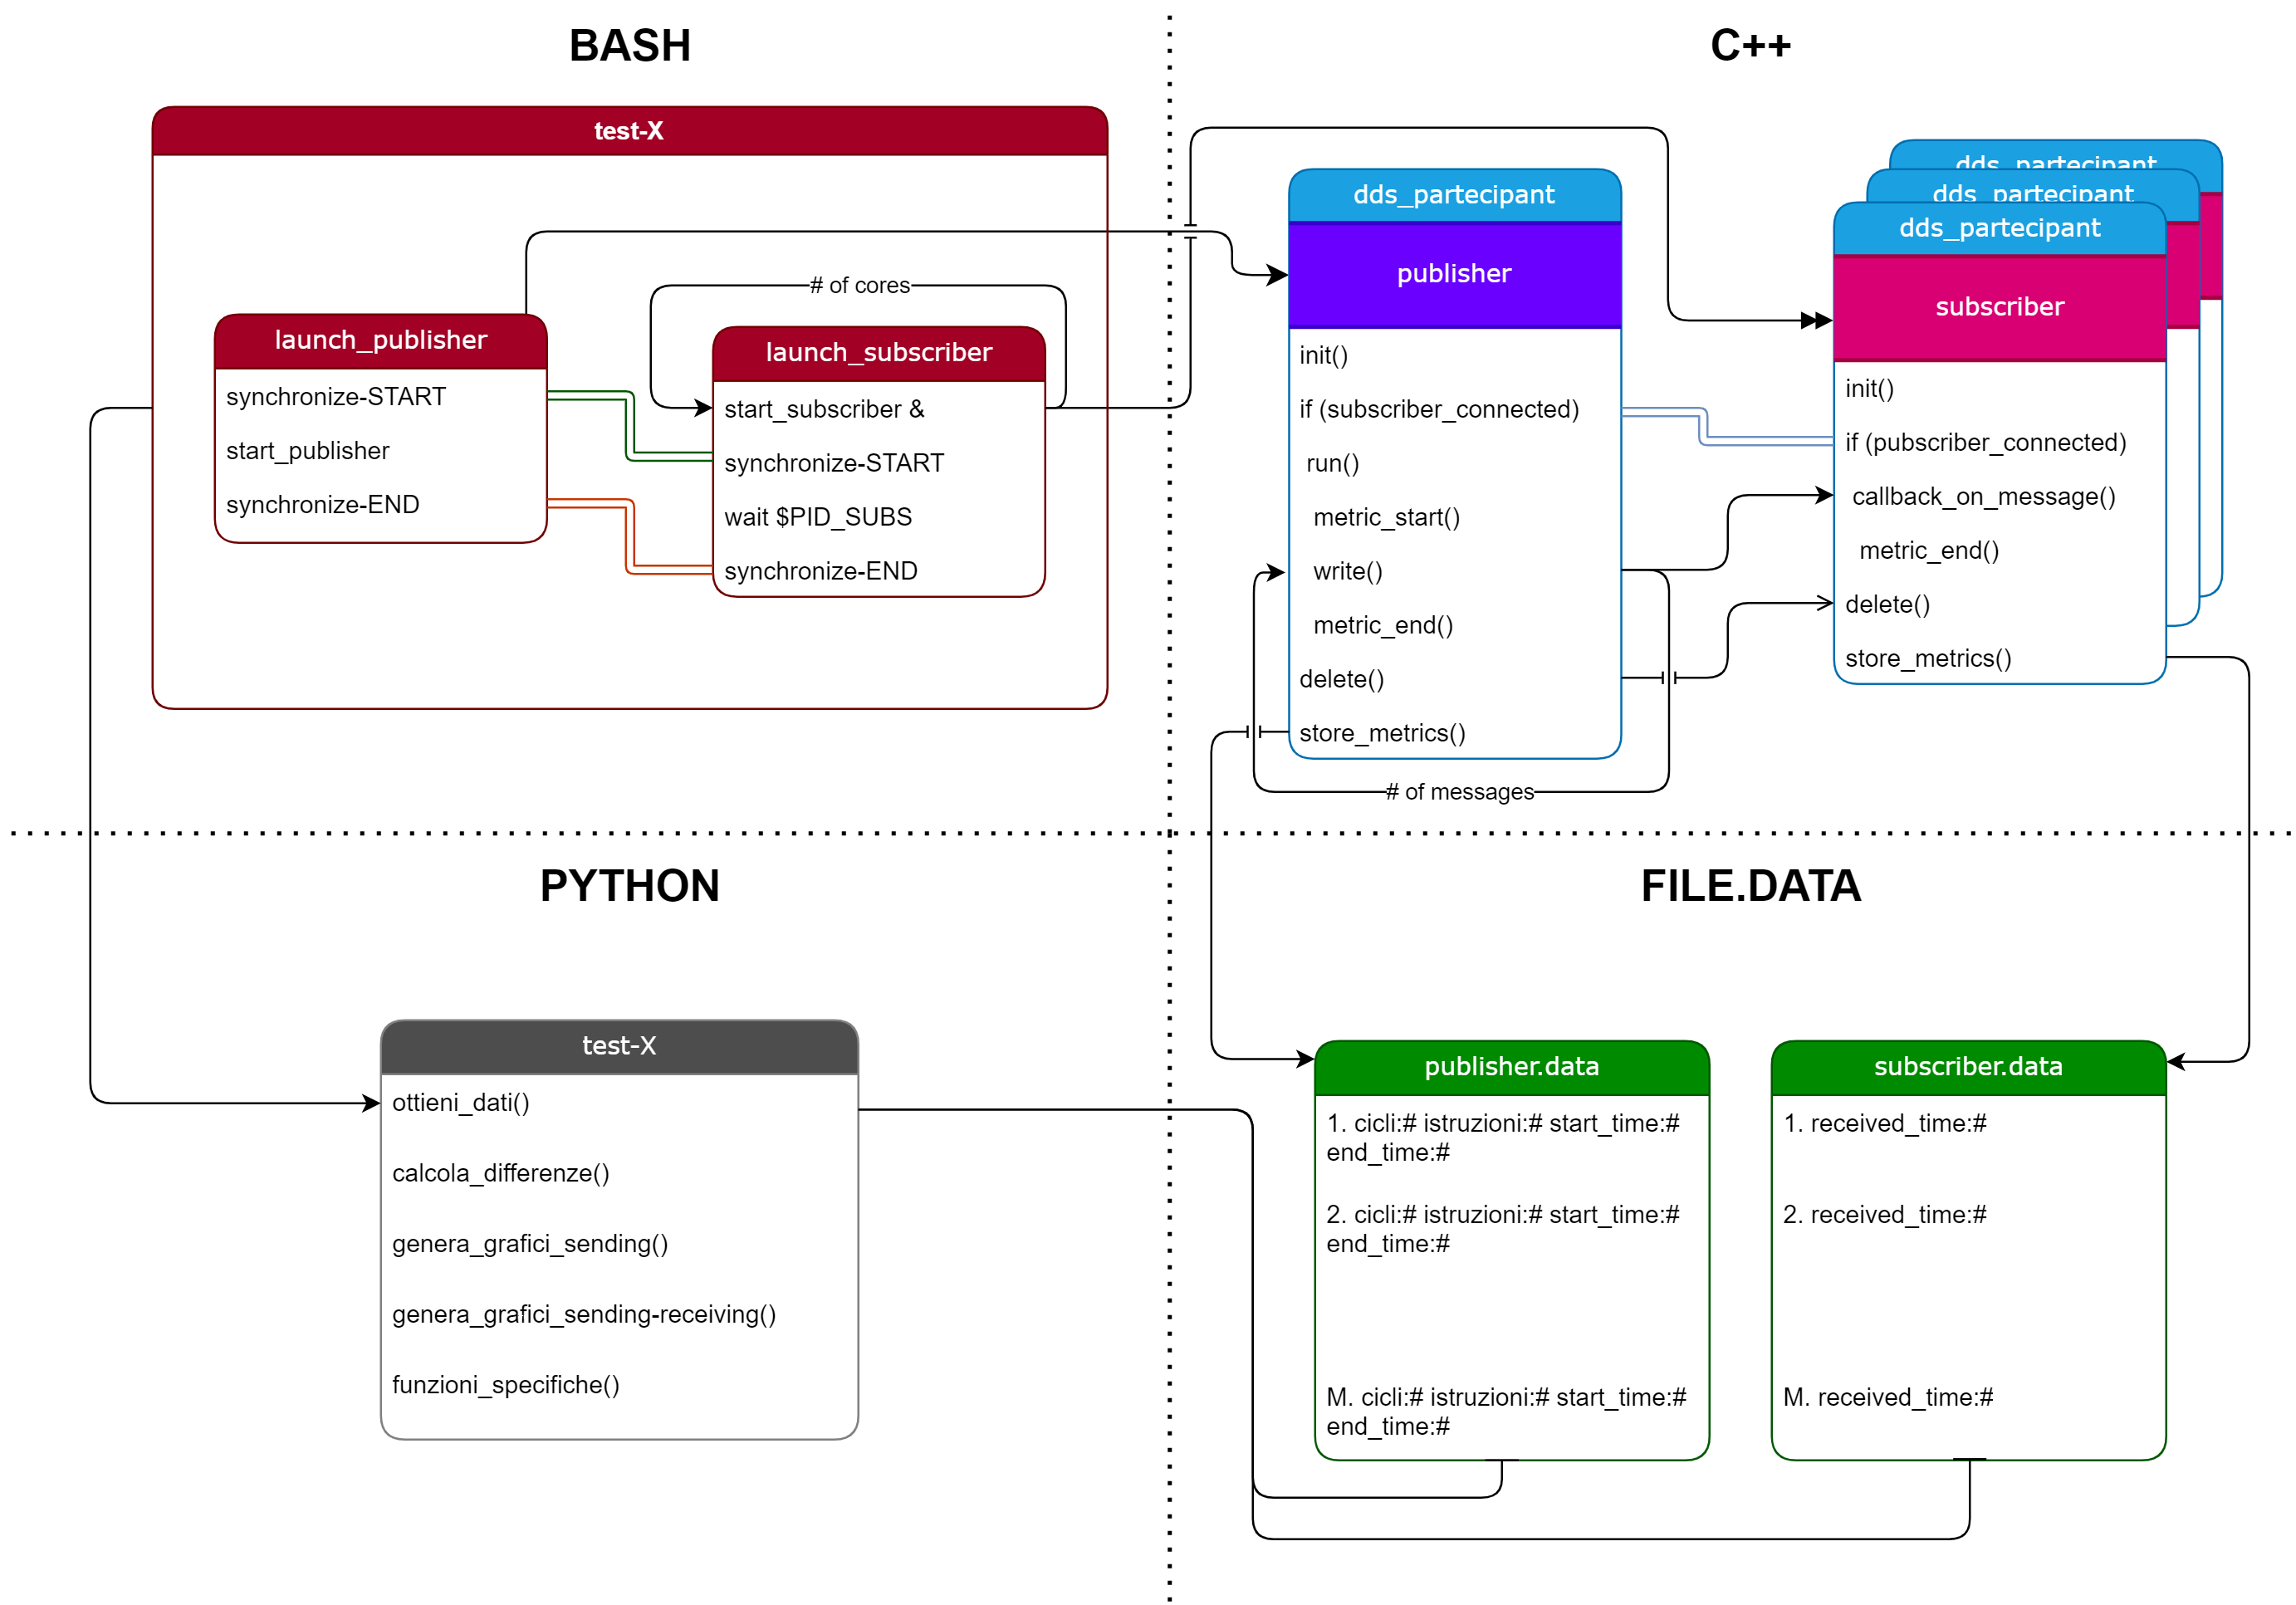
\includegraphics[width=\textwidth]{./img/schema_test_globale.drawio.png}
    \caption{Struttura test} %TODO: add readtsc, istr
    \label{fig:schema_global}
\end{figure}

\subsection{Bash}\label[Sezione]{sec:Shell}
Vista la necessità di lanciare diversi publisher e diversi subscriber ogni volta con dei parametri variabili è stato conveniente usare programmi di scripting come \gls{Bash}. Infatti questi gestivano i parametri variabili da passare agli attori, inizializzavano le variabili d'ambiente, decidevano quali core dovevano essere utilizzati da ogni partecipante (task-setaffinity) e mantenevano sincronizzati i test per evitare che alcuni attori fossero inizializzati troppo presto. Infine ripulivano e ordinavano i dati una volta terminato i test ed andavano ad eseguire gli script python che processavano i dati, nelle cartelle corrette.
\subsection{C++}
E' stato scelto di utilizzare direttamente l'implementazione DDS invece che il già citato \emph{Ros middlware} [\ref{SSEC:rosiface}] per i seguenti motivi:
\begin{itemize}
    \item Potenzialità: ROS mette a disposizione solo alcuni degli strumenti resi disponibili dallo strato DDS, andando a limitare la possibilità di sfruttamento di tutte le impostazioni e QoS di FastDDS;
    \item Flessibilità: Per andare a definire delle strutture dati di ROS, al fine di scambiare messaggi DDS usando il middleware offerto, era necessario creare diverse strutture dati che combaciassero con le interfacce ROS;
    \item Comodità: Implementare completamente \emph{rmw\_dds\_common} richiedeva un impegno e uno studio non indifferente della architettura sottostante a ROS, che seppur ben documentata, sarebbe costata molto tempo in più. 
\end{itemize}
E' stato scelto di realizzare una unica implementazione publisher e subscriber dove i valore delle funzionalità che si volevano testare dovevano essere passati come parametro lato bash (\ref{sec:Shell}) in modo da poter avviare tutti i test con gli stessi codici, rendendo più semplice la gestione dei diversi test, e più robusto ad errori dovuti a diverse configurazioni.
\subsubsection*{Struttura}

Per scambiarsi dei messaggi all'interno di infrastruttura basata su DDS, sono necessari: (i) un topic, (ii)un publisher ed (iii) un subscriber. Inoltre nel topic è necessario definire il tipo dato o struttura di dati che si va a scambiare. La struttura che si è scelta di utilizzare per i test è stata la seguente:
\begin{verbatim}
    struct DDSTest
    {
        unsigned long index;
        std::string message;
    };
\end{verbatim}
Dove index era necessario per definire una corrispondenza stretta tra i messaggi inviati e quelli ricevuti, mentre la stringa era comoda per definire un oggetto di dimensione molto variabile (anche dinamicamente durante i test).

Una volta studiata la documentazione ufficiale di eProsima FastDDS, è stato sviluppato un codice in grado di integrare tutte le funzionalità di DDS ed alcuni strumenti per l'ottenimento di metriche precedentemente concordate con Cineca\cite{TODO}. Nello specifico sono state scelte:
\begin{itemize}
    \item Tempo di invio
    \item Istruzioni Perf-Event per invio
    \item Cicli TSC (read\_tsc) per invio
    \item Tempo di invio e ricezione
\end{itemize}
\subsection{Lettura TSC}
Il Time Stamp Counter, è un registro a 64 bit, presente nella maggior parte dei processori moderni. Il registro fornisce informazioni sul tempo, in termini di cicli di clock del processore, e viene spesso utilizzato per effettuare misure di queste metriche. Per leggere questo valore, che viene fatto prima e dopo l'istruzione da misurare, è necessario eseguire la seguente istruzione:
\begin{verbatim}
    unsigned int lo, hi;
    __asm__ __volatile__ ("rdtsc" : "=a" (lo), "=d" (hi));
    return ((uint64_t)hi << 32) | lo; 
\end{verbatim}
\emph{rdtsc} è l'istruzione \gls{assembly} per leggere il registro Timestamp Counter, =a (lo) e =d (hi) sono i vincoli di output che specificano come i risultati dell'istruzione rdtsc devono essere restituiti al programma. In lo ("=a") viene riportat il valore a 32 bit meno significativo ed in hi, il valore a 32 bit più significativo.

\subsection{Conteggio istruzioni}
Per le istruzioni invece è stato usato lo strumento \textbf{Perf}, un software offerto da Linux ed incluso anche nel suo \gls{Kernel}, per la profilazione delle performance tramite i \emph{performance\_counter}. Questa suite è estremamente avanzata e permette di ottenere delle metriche specifiche senza troppa difficolta. In questo caso è stata usata una chiamata alla libreria \textbf{perf\_event} nel codice per il valore \emph{PERF\_COUNT\_HW\_INSTRUCTIONS}.

\subsection{Ottenimento dei tempi}
In sistemi molto complessi come può essere considerato un supercalcolatore, la gestione degli orologi è tutt'altro che banale. Infatti dopo aver deciso una tra le tante politiche di sincronizzazione disponibile come centralizzata, distribuita, GPS e tante altre, è necessario applicarle e continuare a tenere questi orologi sullo stesso tempo assoluto. Nei sistemi utilizzati in questo progetto, ed in particolare nei sistemi \ref{table:hpc-cineca}, lo strumento adottato è Network Time Protocol (fornito da \gls{ntpd}). Quest'utlimo ogni intervallo di tempo impostato, va a rendere disponibile ai vari nodi ed ai rispettivi orologi locali un tempo di riferimento che ha la funzione di punto fisso. Questo intervallo è normalmente fissato ogni 1024s, ma non disponendo dei diritti necessari ad utilizzarlo, non mi è stato possibile recuperare l'informazione.

Detto questo, per ottenere le differenze di tempi su sistemi Linux, è ricorrente utilizzare una funzione chiamata \textbf{clock\_gettime()} che restituisce il tempo istantaneo alla chiamata. Se si esegue la differenza tra due diverse clock\_gettime(), si ottiene il tempo trascorso tra queste due.
Per questa funzione è possibile ottenere diverse metriche tra cui:
\begin{itemize}
    \item CLOCK\_REALTIME: ottiene il tempo assoluto, sincronizzato dei vari sistemi da ntpd
    \item CLOCK\_MONOTONIC: ottiene un tempo relativo, da un punto non preciso dall'avvio del sistema
    \item CLOCK\_MONOTONIC\_RAW: come sopra, ma non influenzato da ntpd
    \item CLOCK\_PROCESS\_CPUTIME\_ID: timer dei processori ad alta risoluzione
    \item CLOCK\_THREAD\_CPUTIME\_ID: tempo dei thread dei processori
\end{itemize}
Tra queste è stato utilizzato il MONOTONIC, visto che il REALTIME con aggiornamenti di ntpd di 1024s subisce variazioni di alcuni millisecondi\cite{ntpd}, di gran lunga superiore all'ordine di grandezza da misurare (microsecondi, a volte anche nanosecondi). Inoltre dato che per eseguire i test è stato usato un solo sistema per volta (o Cineca, o E4) MONOTONIC\_RAW non era necessario (anche in caso di aggiornamento ntp, viene diffuso in egual modo su tutti i nodi).
Il problema di usare la MONOTONIC, è che su sistemi con orologi diversi, questi sono sfasati di diverse migliaia di secondi. E' stato necessario aggirare questo problema, e per farlo sono stati usati 2 approcci completamente diversi:
\begin{itemize}
    \item Sincronizzazione dei nodi
    \item RTT
\end{itemize} 

\noindent Entrambi i tentativi verranno approfonditi nelle successive sezioni \ref{TODO}


\subsubsection{UML}
Lo schema UML di funzionamento degli attori DDS è riassunto e schematizzato dalla figura \ref{fig:uml}
\begin{figure}[H]
    \centering
    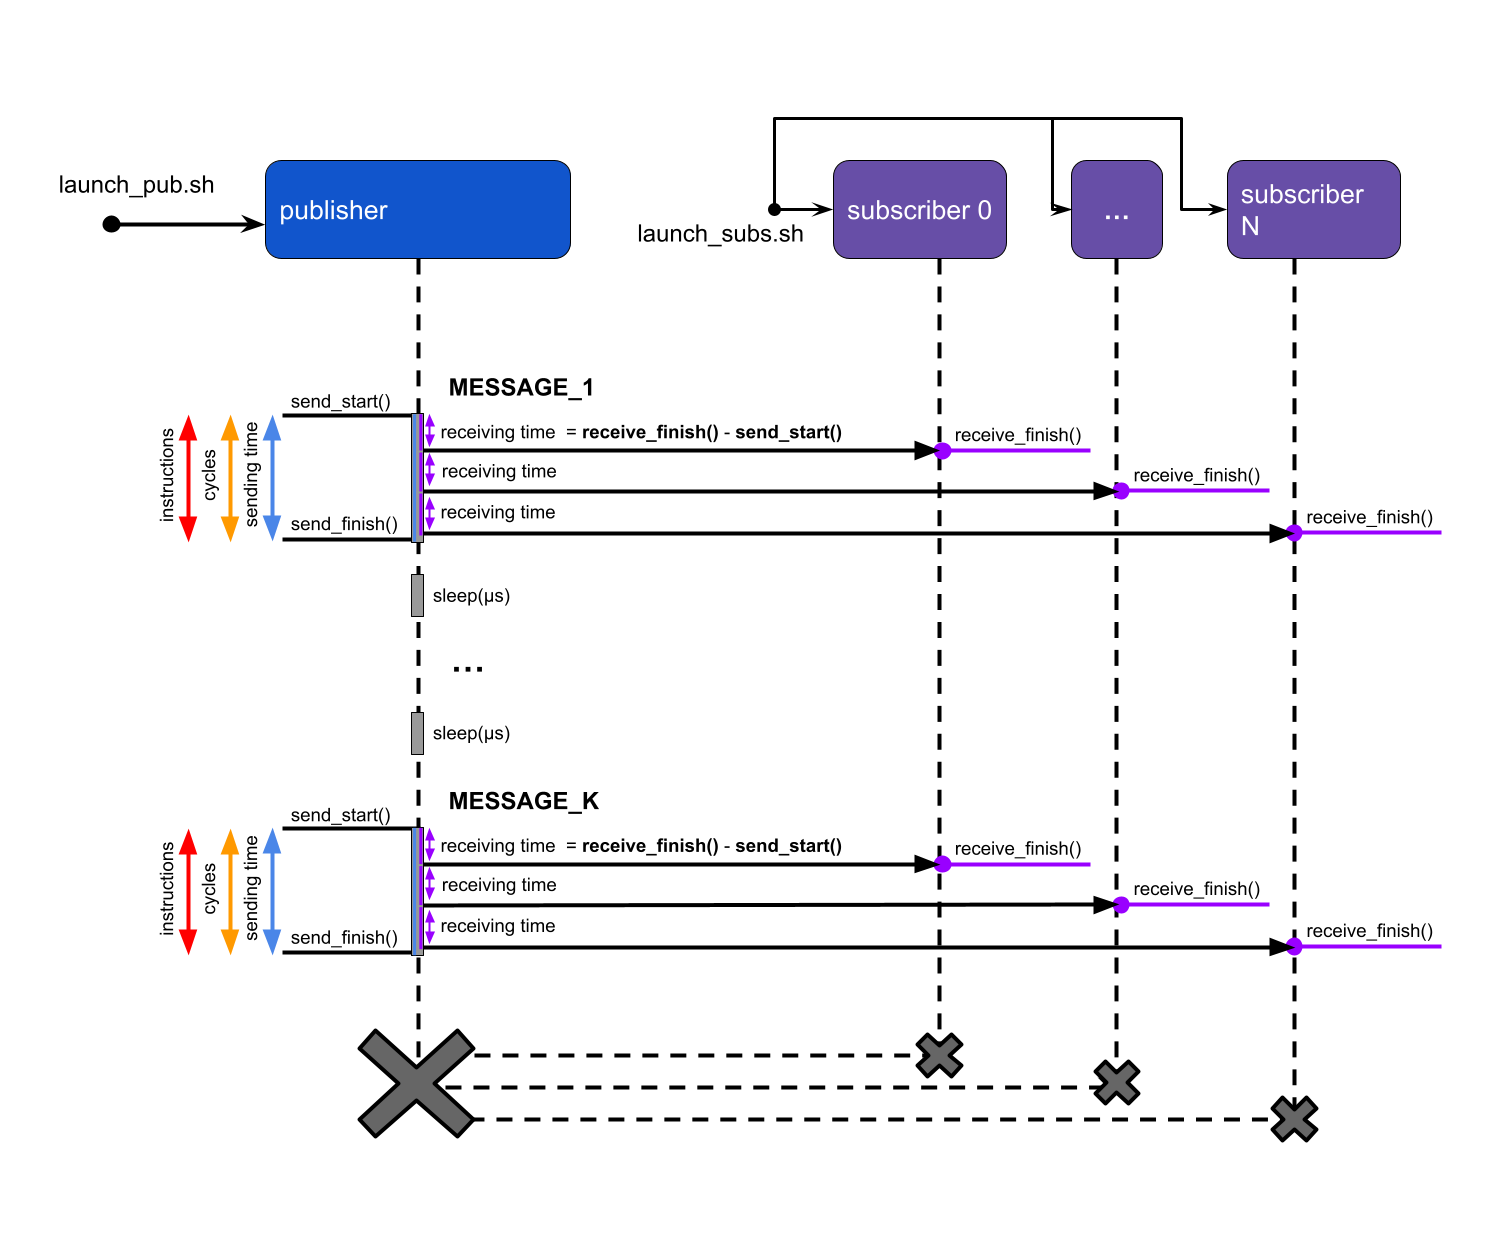
\includegraphics[width=\textwidth]{./img/umel-send-receive.png}
    \caption{Schema UML} %TODO: typo on receiving time = recIVE
    \label{fig:uml}
\end{figure}

In particolare nel Publisher \ref{actor:publisher} prima e dopo la chiamata a funzione di write() %TODO: inserire nella tesi?
si sono presi i valori tempo-invio, istruzioni, e TSC, mentre al lato ricevente, di Subscriber \ref{actor:subscriber} è stato preso il tempo al momento dell'arrivo del messaggio. Segue uno schema uml della base di ognuno dei test.

%TODO: se serve approfondire TSC, e metriche eseguite prima e dopo

\section{DataMiners}
Considerando che ogni publisher genera 10K messaggi da inviare a 48 subscriber, per ogni protocollo di trasporto, e in alcuni casi in partizioni differenti si è arrivato ad avere per ogni test fino a $1'960'000$ messaggi scambiati e le relative metriche per ogni messaggio da processare. 
Gli script python sono stati utili a organizzare e processare tutti i dati prodotti dai vari test. Inoltre sono stati fondamentali per poter generare tutti i grafici che sono stati in questa tesi.

\section{Sincronizzazione}\label{sec:timesync}
Una delle prime soluzioni che è stata provata, è stata quella di sincronizzare gli orologi locali dei diversi nodi tramite l'utilizzo di librerie sviluppate per la programmazione parallela come Message Passing Interface (MPI). Quest'ultimo è un protocollo di comunicazione molto utilizzato nei sistemi HPC per la programmazione parallela.
Nello specifico è stata utilizzata una funzionalità chiamata MPI\_barrier, che permette di bloccare i processi, fino all'arrivo di un punto in comune, dopo il quale tutti procedono insieme. Questo serve per sincronizzare i processi tra di loro, ma non è ideata nello specifico per sincronizzare gli orologi. Gli strumenti strumenti utili alla mera sincronizzazione dei tempi dei nodi sono altri, come il già citato Network Time Protocol,
ma essendo ntpd un servizio di amministrazioni non è stato possibile interagirci e quindi usarli. Nella figure \ref{fig:sync_time_shift1} \ref{fig:sync_time_shift2} \ref{fig:sync_time_shift3} sono stati riportati i dati ottenuti grazie a questo meccanismo.

\begin{figure}[H]
    \centering
    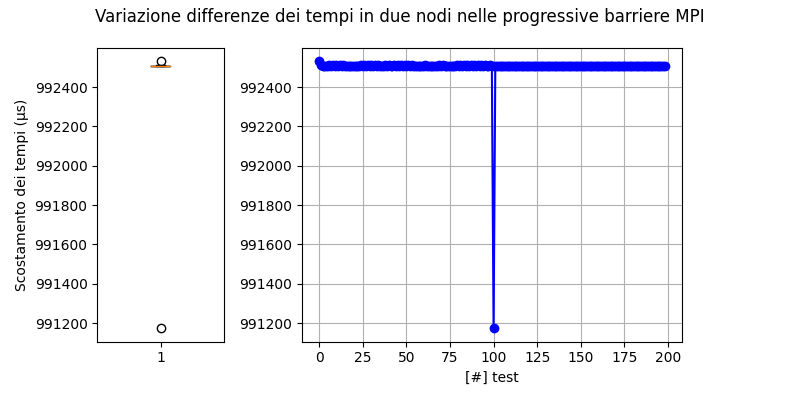
\includegraphics[width=\textwidth]{./results/time_sync_node.png}
    \caption{Scostamento del tempo su nodi diversi}
    \label{fig:sync_time_shift1}
\end{figure}
\begin{figure}[H]
    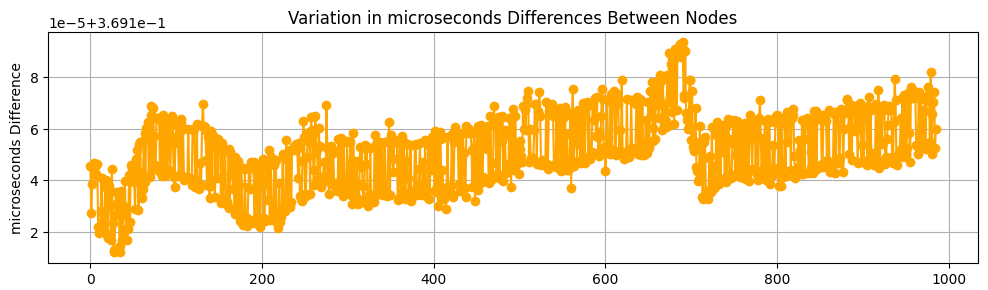
\includegraphics[width=0.99\textwidth]{./results/time_shift_clean.png}
    \caption{Scostamento senza outliers}
    \label{fig:sync_diff_distr2}
\end{figure}
\begin{figure}[H]
    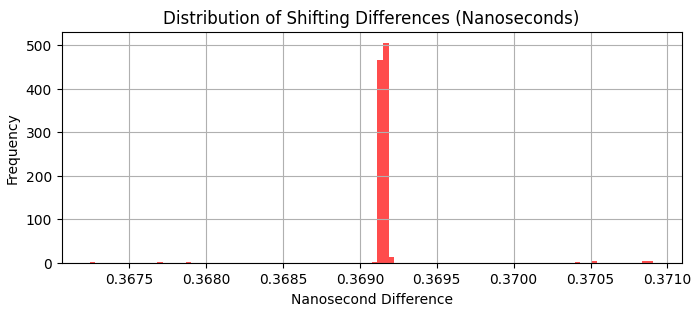
\includegraphics[width=\textwidth]{./results/time_sync_distribution.png}
    \caption{Distribuzione delle differenze}
    \label{fig:sync_diff_distr3}
\end{figure}

Come possibile notare nella figura \ref{fig:sync_time_shift1} nonostante le mpi\_barrier, gli scostamenti di tempo tra 2 nodi durante i diversi tentativi effettuati (1000), cambia notevolmente, arrivando a differenze fino ad un massimo di 290 microsecondi. Questo rende il metodo appena mostrato utilizzabile solo nel caso in cui non sia necessario sapere il tempo assoluto di qualche azione, ma le varianze, che rimarrebbero costanti se si utilizzano sempre gli stessi nodi.


\section{RTT}\label{sec:timeRTT}
Nonostante la sincronizzazione, fosse idealmente il metodo più preciso per ottenere i tempi di invio-rivezione, essendo l'errore possibile dello stesso ordine di grandezza dei tempi di ricezione, per alcuni test si è utilizzato un approccio che non richiedesse sincronizzazione. Il metodo più intuitivo è utilizzare il Round Trip Time (RTT).
Il RTT è un metrica che viene solitamente utilizzata per misurare la latenza di una rete, e si basa sull'idea di calcolare il tempo che intercorre tra lìinvio di un segnale e la ricezione della conferma di arrivo dello stesso. Ovviamente il valore ottenuto risulta nel caso ideale più che raddoppiato vista la necessità di un messaggio di risposta. Nel diagramma \ref{fig:uml} non sarebbe stato possibile condurre questa misura, perchè un subscriber non può inviare un messaggio di risposta.
Per farlo è stato necessario rivedere gli attori coinvolti, ed introdurre in quello che prima venivano chiamati publisher e subscriber, un publisher e un subscriber a testa.
Per semplificarne la comprensione viene riportato lo schema modificato:

\begin{figure}[H]
    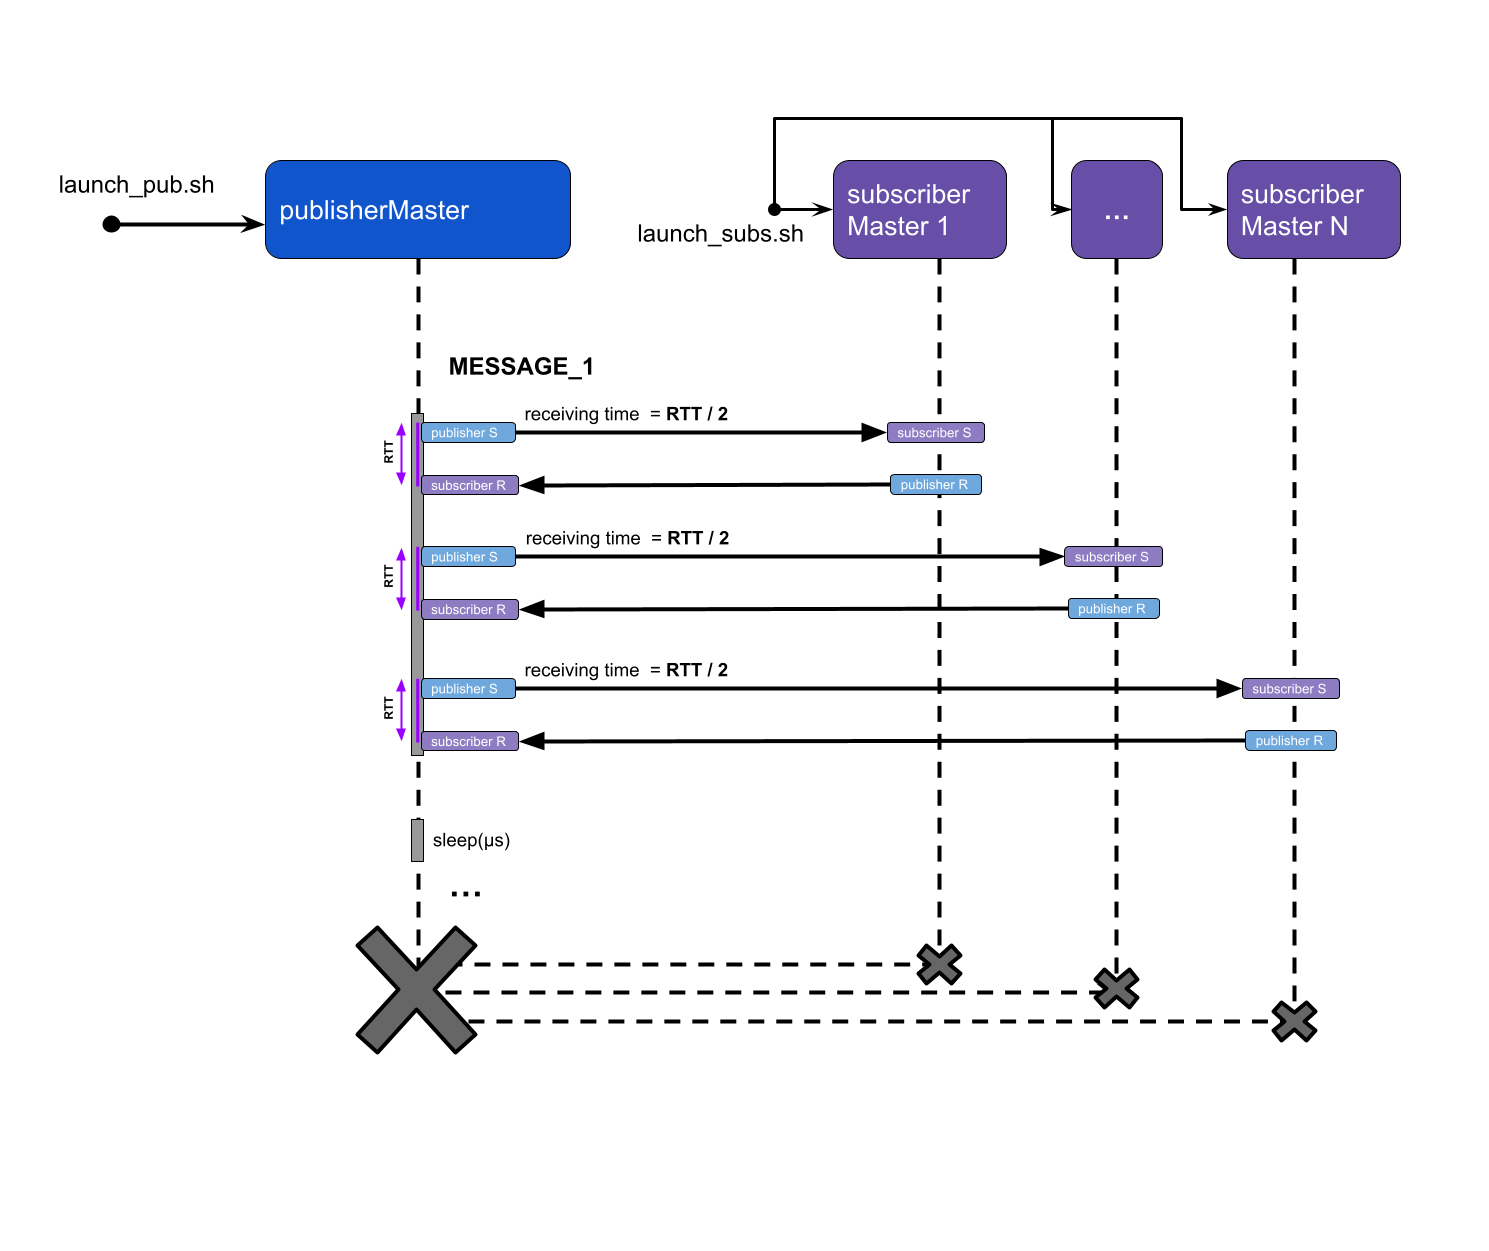
\includegraphics[width=\textwidth]{./img/RTT.png}
    \caption{Schema UML RTT}
    \label{fig:rtt_uml}
\end{figure} 

Ovviamente questo metodo può comportare qualche ritardo intrinseco di dover gestire due entità per ogni attore, ma sono tempi infinitesimali in confronto al tempo necessario per inviare il messaggio su rete (dove è stato usato questo approccio).

\section{Schema}
Sono stati svolti diversi test al fine di trovare un modello ottimale di utilizzo e per la caratterizzazione di DDS, all'interno di sitemi HPC, nel contesto del Power Management. Nello specifico i test sono stati utili a capire il peso che avesse una singola configurazione o modello di utilizzo al fine di trovare quello più adeguato per una futura implementazione. I test effettuati sono:

\begin{itemize}
    \item test-1: protocollo di comunicazione
    \item test-2: partizioni e wildcards
    \item test-3: throughput
\end{itemize}


Al fine di condurli nel modo più trasparente e corretto possibile sono stati resi pubblici \cite{mygit} tutti i codici utilizzati durante lo svolgimento di questi test. %TODO5O: riordinare & documentare git

\subsection{Test-1}
In DDS ed in particolare nel layer sottostante di RTPS, per scambiare messaggi anche tramite rete, e non solo nello stesso nodo, è possibile scegliere come mezzo diversi tipi di protocolli:

\begin{itemize}
    \item udp: fornisce due versioni v4 e v6 e importa l'omonimo protocollo di trasporto
    \item tcp: fornisce due versioni v4 e v6 e importa l'omonimo protocollo di trasporto
    \item udp-multicast: una versione modificata del semplice udp, dove tutti i subscriber collegati allo stesso topic, hanno un indirizzo comune di ricezione dei dati, permettendo così al publisher di inviare un singolo messaggio che viene condiviso tra tutti i subscriber  % TODO: uml
    \item shared-memory: analogo al metodo precedentemente, ma invece di utilizzare un indirizzo IP, viene utilizzato un indirizzo di memoria. E' possibile solo quando i due processi che comunicano sono sullo stesso nodo, con memoria condivisa.
\end{itemize}

Nel primo test si è valutata la differenza di queste implementazioni utilizzando la rete infiniband \ref{table:hpc} su diversi nodi di un supercalcolatore. 

\subsection{Test-2}
Un concetto fondamentale nelle comunicazioni tra attori con gerarchie diverse, in sistemi con diverse centinaia di migliaia di entita, come cluster, nodi, processori, workflow, job (etc.), sono le possibilità di instradare, segmentare e rendere gerarchiche le comunicazioni. Come spiegatolo nel capitolo \ref{Chapter:dds} in DDS ci sono diversi strumenti disponibili per farlo. Tra di loro differiscono per alcuni aspetti, come flessibilità, costo (in performance) e livello di segmentazione.

In questo test si è valutata la differenza in termini di performance dei diversi strumenti, con un particolare focus sulle partizioni e le wildcards rese disponibili in esso.

\subsubsection*{Dominio} 
Il dominio è la segmentazione di più "forte" e di più alto livello. Va a partizionare gli attori presenti in un dominio in modo del tutto fisico (cambiando per ogni dominio porte e indirizzi di comunicazione) e per nulla flessibile. Per cambiare il dominio è necessario distruggere e creare di nuovo il partecipante. Inoltre il dominio non permette nessun tipo di gerarchia.
    
\subsubsection*{Topic}
All'interno di un dominio i topic definiscono il metodo principale di instradamento dei messaggi, essendo però limitato dal tipo di messaggio che si vuole inviare. Infatti topic diversi supportano tipi di dato diversi, e non sono modificabili a run-time. %TODO: glossario
Inoltre il topic non permette gerarchie ed è difficilmente modificabile a run-time

\subsubsection*{Partizione}
Questo strumento risulta molto interessante, in quanto all'interno di un topic permette di definire gerarchie (è possibile sottoscriversi a più partizioni contemporaneamente), definisce wildcards e crea una segmentazione virtuale. Inoltre è facilmente modificabile a run-time.

\subsubsection{Wildcards}
Le wildcards sono un costrutto appartenente alle partizioni, che permette di definire dei pattern testuali sulla base del quale vengono instradati i messaggi. Un esempio può essere \textit{Node*} che va a corrisponde a tutti i messaggi sotto il topic precedentemente definito, a tutte le partizioni che iniziano con Node.
%TODO: Schema test 2

\begin{figure}[H]
    \centering
    %TODO DA INSERIRE WILDCARDS costi
    %\includegraphics[width=\textwidth]{./results/}
\end{figure}


\subsection{Test-3}
Nel test-3 si è voluto misurare il throughput e la bandwidth massima per ciascun protocollo. Per calcolarlo sono stati usati i seguenti dati:

\begin{table}[H]
    \begin{center}
    \begin{tabular}{l|l}
        \hline
        \textbf{Parametri} & \textbf{Valore}\\
        \hline
        [\#] publisher & 1 \\
        \hline
        [\#] subscriber & 40 \\
        \hline
        [\#] messaggi scambiati (per attore) & 10 000 \\
        \hline
        Dimensione del messaggio & 16 Byte \\
        \hline
    \end{tabular}
    \end{center}
    \caption{Valori usati per il test 3}\label{table:hpc-cineca}
    \end{table}
    
